\item{Con cualesquiera dos variables $x$, $y$ tenemos:
\begin{equation}
H\left ( x,y \right )\leq H\left ( x \right )+H\left ( y \right )
\end{equation}
con igualdad si (y solo si) $x$ y $y$ son independientes, por ejemplo,
$p\left ( x,y \right )=p\left ( x \right )p\left ( y \right )$
(adem\'as posiblemente un conjunto de puntos de probabilidad cero).}
\item{Considere una operaci\'on de promedio generalizada del siguiente tipo:
\begin{equation}
{p}'\left ( y \right )=\int a\left ( x,y \right )p\left ( x \right ) \diff x 
\end{equation}
con
\begin{equation}
\int a\left ( x,y \right ) \diff x =\int a\left ( x,y \right ) \diff y =1, 
\,  a\left ( x,y \right )\geq 0
\end{equation}
Entonces la entrop\'ia de la distribuci\'on promediada ${p}'\left ( y
\right )$ es igual o mayor a la distribuci\'on original $p\left
( y \right )$.}
\item{Tenemos:
\begin{equation}
H\left ( x,y \right )=H\left ( x \right )+H_{x}\left ( y \right )=H\left ( y \right )+H_{y}\left ( x \right )
\end{equation}
y
\begin{equation}
H_x{}\left ( y \right )\leq H\left ( y \right ).
\end{equation}}
\item{Dejamos $p\left ( y \right )$ ser una distribuci\'on unidimensional. La forma de $p\left ( y \right )$ dando una m\'axima entrop\'ia sujeto a la condici\'on de que la desviaci\'on est\'andar de $x$ es fija en $\sigma $ es Gaussiana. Para demostrar \'esto debemos maximizar:
\begin{equation}
H\left ( x \right )=-\int p\left ( x \right )\log p\left ( x \right ) \diff x 
\end{equation}
con
\begin{equation}
\sigma^{2}=\int p\left ( x \right )x^{2} \diff x  \:\:\:\:\: \textup{y} \:\:\:\:\: 1=\int p\left ( x \right ) \diff x 
\end{equation}
como l\'imites. \'Esto requiere, por el c\'alculo de variaciones, maximizar:
\begin{equation}
\int \left [ -p\left ( x \right ) \log p\left ( x \right ) + \lambda p\left ( x \right ) x^{2} + \mu p\left ( x \right )\right ] \diff x 
\end{equation}

La condici\'on para \'esto es
\begin{equation}
-1-\log p\left ( x \right )+\lambda x^{2}+\mu =0
\end{equation}
y consecuentemente (ajustando las constantes para satisfacer los l\'imites)
\begin{equation}
p\left ( x \right )=\frac{1}{\sqrt{2\pi \sigma }}e^{-\left ( x^{2}/2\sigma ^{2} \right )}
\end{equation}
Del mismo modo en $n$ dimensiones, supongamos que los momentos de
segundo orden de $p\left ( x_{1}, \ldots ,x_{n} \right )$ son fijos en
$A_{ij}$:
\begin{equation}
A_{ij}=\int \cdots \int x_{i}x_{j}p\left ( x_{1}, \ldots ,x_{n} \right ) \diff x _{1}\cdots  \diff x_{n}
\end{equation}
Entonces la m\'axima entrop\'ia ocurre (por un c\'alculo similar)
cuando $p\left ( x_{1}, \ldots ,x_{n} \right )$ es la distribuci\'on
Gaussiana $n$ dimensional con los momentos de segundo orden $A_{ij}$.}
\item{La entrop\'ia de una distribuci\'on Gaussiana undimensional cuya desviaci\'on estandar es $\sigma$ est\'a dada por
\begin{equation}
H\left ( x \right )=\log \sqrt{2\pi e\sigma }
\end{equation}
\'Esta es calculada de la siguiente forma
\begin{equation}
\begin{array}{rcl}
p\left ( x \right ) &=&
\frac{1}{\sqrt{2\pi \sigma }}e^{-\left ( x^{2}/2\sigma ^{2} \right )} \\
-\log p\left ( x \right )
&=& 
\log \sqrt{2\pi \sigma }+\frac{x^{2}}{2\sigma ^{2}} \\
H\left ( x \right )
&=&
-\int p\left ( x \right )\log p\left ( x \right ) \diff x \\
&=&
\int p\left ( x \right )\log \sqrt{2\pi \sigma } \diff x +\int p\left ( x \right )\frac{x^{2}}{2\sigma ^{2}} \diff x  \\
&=& \log \sqrt{2\pi \sigma }+\frac{\sigma }{2\sigma ^{2}} \\
&=& \log \sqrt{2\pi \sigma }+\log \sqrt{e} \\
&=&\log \sqrt{2\pi e \sigma }
\end{array}
\end{equation}
Asimismo, la distribuci\'on Gaussiana n-dimensional con una forma cuadr\'atica asociada $A_{ij}$ est\'a dada por:
\begin{equation}
p\left ( x_{1}, \ldots ,x_{n} \right )=\frac{\left | a_{ij} \right |^{\frac{1}{2}}}{\left ( 2\pi  \right )^{n/2}}\exp \left ( -\frac{1}{2} \sum a_{ij}x_{i}x_{j} \right)
\end{equation}
y la entrop\'ia puede se calculada como:
\begin{equation}
H=\log \left ( 2\pi e \right )^{n/2}\left | a_{ij} \right |^{-\frac{1}{2}},
\end{equation}
donde $\left |a_{ij}  \right | $ es la determinante cuyos elementos son $a_{ij}$.}
\item{Si $x$ es limitada a una media l\'inea ($p\left ( x \right )=0$ para $x\leq0$ y el primer momento de $x$ es fijado en $a$:
\begin{equation}
a=\int_{0}^{\infty}p\left ( x \right )x \diff x,
\end{equation}
entonces la m\'axima entrop\'ia ocurrir\'a cuando
\begin{equation}
p\left ( x \right )=\frac{1}{a}e^{-\left ( x/a \right )}
\end{equation}
y es igual a $\log ea$.}
\item{Hay una importante diferencia entre la entrop\'ia continua y discreta. En el caso discreto la entrop\'ia mide de un modo absoluto la aleatoriedad de la variable de oportunidad. En el caso continuo la medici\'on es relativa al sistema de coordenadas. Si cambiamos las coordenadas la entrop\'ia cambiar\'a de forma general. En efecto, si cambiamos las coordenadas $y_{1} \dots y_{n}$ la nueva entrop\'ia estar\'a dada por:
\begin{equation}
H\left ( y \right )=\int \cdots \int p\left ( x_{1}, \ldots ,x_{n} \right )J\left ( \frac{x}{y} \right )\log p\left ( x_{1}, \ldots ,x_{n} \right )J\left ( \frac{x}{y} \right ) \diff y _{1}\cdots  \diff y _{n},
\end{equation}
donde $J\left ( \frac{x}{y} \right )$ es el Jacobiano de la transformaci\'on de las coordenadas. En la ampliaci\'on de los logaritmos y cambiando las variables a $x_{1}\dots x_{n}$, obtendremos:
\begin{equation}
H\left ( y \right )=H\left ( x \right )-\int \cdots \int p\left ( x_{1}, \ldots ,x_{n} \right )\log J \left ( \frac{x}{y} \right ) \diff x _{1}\cdots  \diff x _{n}
\end{equation}
Por consiguiente, la nueva entrop\'ia es la vieja entrop\'ia menos el logaritmo esperado del Jacobiano. En el caso continuo la entrop\'ia puede considerarse una medida de aleatoriedad relativa a un est\'andar asumido, es decir, el sistema de coordenadas elegido con cada peque\~no elemento de volumen $dx_{1}\dots dx_{n}$ dado el mismo peso. Cuando cambiamos el sistema de coordenadas, la entrop\'ia en el nuevo sisema mide la aleatoriedad cuando a elementos de volumen iguales $dy_{1}\dots dy_{n}$ en el nuevo sistema se les da el mismo peso.

A pesar de esta dependencia en el sistema de coordenadas, el concepto de entrop\'ia es tan importante en el caso continuo como en el caso discreto. \'Esto se debe al hecho de que los conceptos derivados de la tasa de informaci\'on y la capacidad del canal dependen de la diferencia de ambas entrop\'ias y esta diferencia no depende del marco de coordenadas, cada uno de los dos terminos ser\'an cambiados por la misma cantidad.
La entrop\'ia de una distribuci\'on continua puede ser negativa. La escala de medici\'on establece un zero arbitrario correspondiente a una distribuci\'on uniforme en una unidad de volumen. Una distribuci\'on que es m\'as limitada que \'esto tiene menos entrop\'ia y ser\'a negativa. Las tasas y capacidades ser\'an, sin embargo, siempre no negativas.}
\item{Un caso particular de cambio de coordendas es la transformaci\'on lineal
\begin{equation}
y_{j}=\sum_{i}^{\:}a_{ij}x_{i}.
\end{equation}
En este caso el Jacobiano es simplemente la determinante $\left | a_{ij} \right |^{-1}$, y
\begin{equation}
H\left ( y \right )=H\left ( x \right )+\log\left | a_{ij} \right |.
\end{equation}
En el caso de la rotaci\'on de coordenadas (o cualquier medici\'on preservando la transformaci\'on) $J=1$ y $H\left ( y \right ) = H\left ( x \right )$.}
\end{enumerate}

\clearpage

\chapter{Entrop\'ia en un conjunto de funciones}
\label{sec:21}

Considere un conjunto de funciones erg\'odico limitado a una cierta
banda de ancho $W$ ciclos por segundo. Dejar
\begin{equation}
p\left ( x_{1}, \ldots ,x_{n}\right )
\end{equation}
ser la funcion de distribuci\'on de densidad para amplitudes $x_{1}\dots x_{n}$ en $n$ puntos sucesivos de muestra. Definimos la entrop\'ia del conjunto por grado de libertad como:
\begin{equation}
{H}'=-\lim_{n\rightarrow \infty }\frac{1}{n}\int \cdots \int p\left ( x_{1}, \ldots ,x_{n}\right ) \log p\left ( x_{1}, \ldots ,x_{n}\right ) \diff x _{1} \ldots  \diff x _{n}
\end{equation}
Tambi\'en definiremos la entrop\'ia $H$ por segundo dividiendo, no por $n$, sino por el tiempo $T$ en segundos para $n$ muestras. Desde que $n=2TW$, $H=2W{H}'$.


Con un blanco ruido t\'ermico $p$ es Gaussiano, tenemos:

\begin{equation}
{H}'=\log \sqrt{2\pi eN}
\end{equation}
\begin{equation}
H=W\log 2\pi eN
\end{equation}

Para una determinada potencia media $N$, el ruido blanco tiene la m\'axima entrop\'ia posible. Esto se deduce de las propiedades de maximizar la distribuci\'on Gaussiana se\~nalada arriba.


La entrop\'ia de un proceso estoc\'astico continuo tiene muchas propiedades an\'alogas a ello para procesos discretos. En el caso discreto, la entrop\'ia est\'a relacionada al logartimo de la probabilidad de largas secuencias, y al n\'umero de secuencias razonablemente probables de larga longitud. En el caso continuo se relaciona de una manera simlar al logaritmo de la densidad de probabilidad de una larga serie de muestras, y el volumen de una probabilidad razonablemente alta en el espacio de la funci\'on.


M\'as precisamente, si asumimos que $p\left ( x_{1},\dots ,x_{n} \right )$ continua en todas las $x_{i}$ y para toda $n$, entonces para una suficientemente larga $n$

\begin{equation}
\left | \frac{\log p}{n} - {H}'\right |< \varepsilon 
\end{equation}

para todas las opciones de $\left ( x_{1},\dots ,x_{n} \right )$ aparte de un conjunto cuya probabilidad total es menor, arbitrariamente peque\~na. Lo siguiente forma la propiedad erg\'odica si dividimos el espacio en un gran n\'umero de peque\~nas celdas. La relaci\'on de $H$ a un volumen puede enunciarse como sigue: Bajo las mismas suposiciones consider\'e el espacio n-dimensional correspondiente a $p\left ( x_{1},\dots ,x_{n} \right )$. Dejar $Vn\left ( 	q \right )$ ser el menor volumen en este espacio que incluye en su interior una probabilidad total de $q$. Entonces:

\begin{equation}
\lim_{n\rightarrow \infty }\frac{\log V_{n}\left ( q \right )}{n}={H}'
\end{equation}

dado $q$ no es igual a $0$ o $1$.


Estos resultados muestran que para una gran $n$ existe un volumen bien definido (al menos en el sentido logar\i'itmico) de alta probabilidad, y que dentro de este volumen la densidad de probabilidad es relativamente uniforme (de nuevo en el sentido logar\'itmico).


En el caso del ruido blanco, la funci\'on de distribuci\'on est\'a dada por:

\begin{equation}
p\left ( x_{1}, \ldots ,x_{n}\right )=\frac{1}{\left ( 2\pi N \right )^{n/2}}\exp -\frac{1}{2N}\sum x_{i}^{2}
\end{equation}

Dado que \'este solo depende de $x$, entonces, las superficies de
igual densidad de probabilidad son esferas y la distribuci\'on entera
tiene simetr\'ia esf\'erica. La regi\'on de alta probabilidad es una
esfera de radio $\sqrt{nN}$. Como $n\rightarrow \infty $ la
probabilidad de caer fuera de una esfera de radio $\sqrt{n\left (
  N+\varepsilon \right )}$ se aproxima a cero y $\frac{1}{n}$ veces el
logaritmo del volumen de la esfera se aproxima a $\log \sqrt{2\pi
  eN}$.  En el caso continuo es conveniente no trabajar con la
entrop\'ia $H$ de un conjunto pero con una cantidad derivada la cual
llamaremos potencia de entrop\'ia. Esto es definido como el poder en
el ruido blanco limitado a la misma banda que el original y teniendo
la misma entrop\'ia. En otras palabras, si ${H}'$ es la entrop\'ia de
un conjunto, su potencia de entrop\'ia es:
\begin{equation}
N_{1} = \frac{1}{2\ pi e} \exp 2{H}'.
\end{equation}

En la imagen geom\'etrica esta cantidad de medir el volumen de mayor
probabilidad por el radio al cuadrado de una esfera teniendo el mismo
volumen. Desde que el ruido blanco tiene la m\'axima entrop\'ia para
una potencia dada, la potencia de entrop\'ia de cualquier ruido es
menor o igual a su actual potencia.

\clearpage

\chapter{P\'erdida de entrop\'ia en filtros lineales}
\label{sec:22}

\begin{theorem}
\label{th:14}
Si un conjunto tiene una entrop\'ia $H_{1}$ por grado de libertad en
la banda $W$, y es transmitido a trav\'es de un filtro con
caracter\'isticas $Y\left ( f \right )$, el conjunto de salida
tendr\'a la entrop\'ia
\begin{equation}
H_{2} = H_{1} + \frac{1}{W}\int_{W}^{\:}\log \left | Y\left ( f \right ) \right |^{2}\diff f.
\end{equation}
\end{theorem}

La operaci\'on de un filtro es esencialmente una transformaci\'on
lineal de coordenadas. Si pensamos en los diferentes componentes
frecuentes como el sistema original de coordenadas, los nuevos
componentes frecuentes son meramente los viejos multiplicados por
factores. La matriz de transformac\'on de coordenadas es entonces
esencialmente diagonalizada en t\'erminos de estas coordenadas. El
Jacobiano de las transformaciones es (para los componentes $n$ seno y
$n$ coseno):
\begin{equation}
J=\prod_{i=1}^{n}\left | Y\left ( f_{i} \right ) \right |^{2},
\end{equation}
donde la $f_{i}$ esta igualmente espaciada a trav\'es de la banda
$W$. Esto ocurre en el l\'imite:
\begin{equation}
\exp \frac{1}{W}\int_{W}^{\:}\log \left | Y\left ( f \right ) \right
|^{2} \diff f
\end{equation}

Desde que $J$ es constante, su valor promedio es la misma cantidad y
aplicando el teorema en el cambio de entrop\'ia con un cambio en las
coordenadas, resultar\'a lo siguiente. Podremos redactarlo en
t\'erminos de la potencia de entrop\'ia. As\'i si la potencia de
entrop\'ia del primer conjunto es $N_{1}$ entonces la del segundo
ser\'a
\begin{equation}
N_{1}\exp \frac{1}{W}\int_{W}^{\:}\log \left | Y\left ( f \right )
\right |^{2} \diff f.
\end{equation}

\begin{table}[!ht]
\caption{Gain, entropy power factor and gain in decibels, and the impulse response.}
\label{table1}
\begin{center}
\begin{tabular}{|m{1mm}m{40mm}|m{20mm}|m{15mm}|m{35mm}|}
\hline
\multicolumn{2}{|c|}{\sc Gain} & {\sc Entropy Power Factor} & {\sc Entropy Power Gain in Decibels} & {\sc Impulse Response} \\
\hline
& 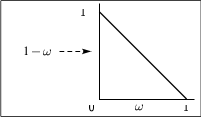
\includegraphics[width=40mm]{./Imagenes/Table11.png} & $\frac{1}{e^2}$ & $-8.69$ & $\frac{\sin^2(t/2)}{t^2 / 2}$ \\
\hline
& 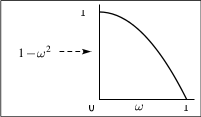
\includegraphics[width=40mm]{./Imagenes/Table12.png} & $\left (\frac{2}{e}  \right )^{4}$ & $-5.33$ & $2\left [ \frac{\sin t}{t^3} - \frac{\cos t}{t^2} \right ]$ \\
\hline
& 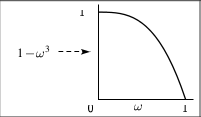
\includegraphics[width=40mm]{./Imagenes/Table13.png} & $0.411$ & $-3.87$ & $6\left [ \frac{\cos t - 1}{t^4} - \frac{\cos t}{2t^2} + \frac{\sin t}{t^3} \right ]$ \\
\hline
& 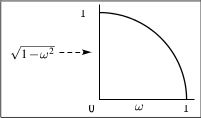
\includegraphics[width=40mm]{./Imagenes/Table14.png} & $\left (\frac{2}{e}  \right )^{2}$ & $-2.67$ & $\frac{\pi }{2} \frac{J_{1}\left ( t \right )}{t}$ \\
\hline
& 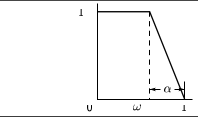
\includegraphics[width=40mm]{./Imagenes/Table15.png} & $\frac{1}{e^{2\alpha}}$ & $-8.69\alpha$ & $\frac{1}{\alpha t^{2}} \left[ \cos \left( 1 - \alpha \right) t - \cos t \right]$ \\
\hline
\end{tabular}
\end{center}
\end{table}

La potencia de entrop\'ia final es la entrop\'ia inicial multiplicada
por la ganancia media geom\'etrica del filtro. Si la ganancia es
medida en $db$, entonces la potencia de entrop\'ia de salida ser\'a
incrementada por la ganancia media aritm\'etica $db$ sobre $W$.

En la tabla 1, la p\'erdida de potencia de entrop\'ia ha sido
calculada (tambi\'en expresada en $db$) para un n\'umero ideal de
ganancias caracter\'isticas. Las respuestas impulsivas de estos
filtros estan dadas tambi\'en por $W = 2 \pi$, con fase en cero.

La p\'erdida de entrop\'ia para otros muchos casos puede ser obtenida
desde estos resultados. Por ejemplo, la del factor de potencia de
entrop\;ia $\frac{1}{e^{2}}$ para el primer caso tambi\'en aplica para
cualquier ganancia caracter\'istica obtenida desde $1-\omega$ por una
medida preservando la transformaci\'on del eje $\omega$. En una
particular ganancia que incrementa linealmente $G \left (\omega
\right) = \omega$, o un ``diente de sierra'' caracter\'istico entre cero y
uno tienen la misma p\'erdida de entrop\'ia. La ganancia rec\'iproca
tiene el factor rec\'iproco. Entonces, $\frac{1}{\omega}$ tiene el
factor $e^{2}$. Aumentando la ganancia a cualquier potencia incrementa
el factor a esta potencia.

\clearpage
